\documentclass[
	a4paper
]{scrreprt}

%%% PACKAGES %%%

% add unicode support and use german as language
\usepackage[utf8]{inputenc}
\usepackage[ngerman]{babel}

% Use Helvetica as font
\usepackage[scaled]{helvet}
\renewcommand\familydefault{\sfdefault}
\usepackage[T1]{fontenc}

% Better tables
\usepackage{tabularx}

% Better enumerisation env
\usepackage{enumitem}

% Use graphics
\usepackage{graphicx}

% Have subfigures and captions
\usepackage{subcaption}

% Be able to include PDFs in the file
\usepackage{pdfpages}

% Have custom abstract heading
\usepackage{abstract}

% Need a list of equation
\usepackage{tocloft}
\usepackage{ragged2e}

% Better equation environment
\usepackage{amsmath}

% Symbols for most SI units
\usepackage{siunitx}

\usepackage{csquotes}

% Clickable Links to Websites and chapters
\usepackage{hyperref}

% Change page rotation
\usepackage{pdflscape}

% Symbols like checkmark
\usepackage{amssymb}
\usepackage{pifont}

\usepackage[absolute]{textpos}

% Glossary, hyperref, babel, polyglossia, inputenc, fontenc must be loaded before this package if they are used
\usepackage{glossaries}
% Redefine the quote charachter as we are using ngerman
\GlsSetQuote{+}
% Define the usage of an acronym, Abbreviation (Abbr.), next usage: The Abbr. of ...
\setacronymstyle{long-short}

% Bibliography & citing
\usepackage[
	backend=biber,
	style=apa,
	bibstyle=apa,
	citestyle=apa,
	sortlocale=de_DE
	]{biblatex}
\addbibresource{Referenzen.bib}
\DeclareLanguageMapping{ngerman}{ngerman-apa}

%%% COMMAND REBINDINGS %%%
\newcommand{\tabitem}{~~\llap{\textbullet}~~}
\newcommand{\xmark}{\ding{55}}

% Define list of equations - Thanks to Charles Clayton: https://tex.stackexchange.com/a/354096
\newcommand{\listequationsname}{\huge{Formelverzeichnis}}
\newlistof{myequations}{equ}{\listequationsname}
\newcommand{\myequations}[1]{
	\addcontentsline{equ}{myequations}{\protect\numberline{\theequation}#1}
}
\setlength{\cftmyequationsnumwidth}{2.3em}
\setlength{\cftmyequationsindent}{1.5em}

% Usage {equation}{caption}{label}
% \indexequation{b = \frac{\pi}{\SI{180}{\degree}}\cdot\beta\cdot 6378.137}{Bogenlänge $b$ des Winkels $\beta$ mit Radius 6378.137m (Distanz zum Erdmittelpunkt am Äquator)}{Bogenlaenge}
\newcommand{\indexequation}[3]{
	\begin{align} \label{#3} \ensuremath{\boxed{#1}} \end{align}
	\myequations{#3} \centering \small \textit{#2} \normalsize \justify }

% Todolist - credit to https://tex.stackexchange.com/questions/247681/how-to-create-checkbox-todo-list
\newlist{todolist}{itemize}{1}
\setlist[todolist]{label=$\square$}

%%% PATH DEFINITIONS %%%
% Define the path were images are found
\graphicspath{{./img/}{./pdf/}}

%%% GLOSSARY ENTRIES %%%
\makeglossaries

%%% DOCUMENT %%%

\begin{document}

\newpage

\pagenumbering{Roman}

\begin{titlepage}
	\begin{textblock*}{5cm}[0,0](15.1cm,1cm)
		
\includegraphics[keepaspectratio,width=5cm]{img/HSLU_Logo}
	\end{textblock*}
	\begin{center}
		\vspace*{5cm}
		\Huge{\textbf{Machbarkeitsstudie}} \\
		\vspace{0.5em}
		\Large{RFID markierte Einzelexemplare}\\
		\vspace{3em}
		\LARGE{Pascal Baumann, Dane Wicki}\\
		\vspace{1em}
		\Large{Betreuer: Martin Jud}\\
		\vfill
		\large{Hochschule Luzern - Departement Informatik}\\
		\large{\today}\\
	\end{center}
	\begin{textblock*}{5cm}[0,0](15.3cm,277mm)
		
\includegraphics[keepaspectratio,width=5cm]{img/FHZ_Logo}
	\end{textblock*}
\end{titlepage}

\renewcommand{\abstractname}{Management Summary}
\begin{abstract}
	In dieser Machbarkeitsstudie werden zu Beginn die Erkenntnisse aus dem gesamten Dokument aufgezeigt, mit der Empfehlung, dass das Projekt durchgeführt werden soll. Anschliessend wird beschrieben, wie das Projekt aufgebaut ist und wo die Kompetenzen liegen. Weiter werden die Beteiligten Parteien erwähnt sowie potenzielle Lieferanten für die RFID HF Hardwareausrüstung identifiziert.
	Anschliessend folgt die Beschreibung des Umfeldes des Projektes, bei welchem näher auf das physische Umfeld der kooperativen Speicherbibliothek eingegangen wird, wie auch auf eine genaue Beschreibung des Problems.
	Darauf folgt eine Bestandsaufnahme, welche Konkurrenz, des mit diesem Projekt zu entwickelnde Produkt, bereits vorhanden ist, sowie der Anschaffungsplan für die Materialien und eine kurze Analyse zur Verfügbarkeit der Arbeitskräfte.
	Weiter werden die technischen Charakteristiken analysiert, welche mit diesem Projekt umgesetzt werden sollen, bei welchen genauer beschrieben wird, welche Hardware zu verwenden ist und wie diese zu positionieren ist. Zudem werden die Vorteile und  Gründe aufgelistet für die Verwendung der beschriebenen Teile.
	In diesem Abschnitt findet sich auch die detaillierte Auflistung für die Kosten der Hardware, sowie der Kosten für weitere Anpassungen.
	Es folgt eine Auflistung der kritischen Punkte des Entwicklungsplanes, bei welchem jeder Punkt näher erläutert wird.
	Nach dem Entwicklungsplan wird auf die Kapitalvoraussetzungen und die Investition eingegangen und anschliessend auf die Betriebskosten.
	Zum Schluss wird analysiert, ob das Projekt wirtschaftlich machbar ist.
\end{abstract}


\tableofcontents

\clearpage
\pagenumbering{arabic}

\chapter{Zusammenfassung der wichtigsten Erkenntnisse}


\chapter{Beschreibung des Projektes}

\section{Natur des Projektes}
Im Rahmen des Projektes soll ein neuer automatischer Arbeitsprozess erstellt werden, welcher sicherstellt, dass mit RFID ausgerüstete Exemplare nicht in einen falschen Behälter platziert werden können. Dieser Arbeitsprozess soll sich in die bestehenden Arbeitsprozesse zur Einlagerung von Exemplaren im Hochregallager der Speicherbibliothek in Büron vollständig integrieren. Dazu soll eine Applikation erstellt werden, welche im Zusammenspiel mit RFID Lesehardware sowie der im Einsatz befindlichen Lagerverwaltungssoftware automatisch im Falle eines deplatzierten Exemplars den Behälter ausschleust. Das Projekt soll im Rahmen einer Bachelorarbeit oder Wirtschaftsarbeit entwickelt werden.

\section{Beteiligte Parteien im Umfeld des Projektes}
Am Projekte sind verschiedene Parteien beteiligt, welche unterschiedliche Auswirkungen und Einflüsse auf das Projekt nehmen können. Es handelt sich primär um folgende Parteien:
\begin{itemize}
	\item Hochschule
	\item kooperative Speicherbibliothek
	\item Stöcklin (Hersteller der Lagerverwaltungssoftware)
	\item Gesetzgeber
\end{itemize}

\section{Struktur des Projektes}
Das Projekt wird durch Studenten des Fachbereiches Informatik in aktiver Zusammenarbeit mit der kooperativen Speicherbibliothek durchgeführt. Währen dieser Durchführung liegt die Entscheidungsgewalt bei den Studenten. Mit Fertigstellung des Projektes wird das Produkt der Speicherbibliothek übergeben. Diese übernimmt anschliessend die Entscheidungsgewalt wie auch die Verantwortung der Wartung sowie Weiterentwicklung des Produktes.

\section{Zielgruppe und Konkurrenten}
Die Zielgruppe ist jede Unternehmung, welches sich zum Ziel gesetzt hat, mehrere mit RFID ausgestattete Objekte indexiert in einem Behältnis zu lagern und das manuelle Deplatzieren eines Objektes in ein falsches Behältnis zu verhindern.
Dazu gehörten Unternehmen mit einem Hochregallager, in welchem sie Exemplare wie zum Beispiel Bücher oder Ordner in Behältnissen lagern und dabei erfassen, welche Exemplare in welchen Behältern gelagert sind.

Es bestehen momentan keine direkten Konkurrenzprodukte, welche verschiedene Exemplare in einem Behältnis auffinden können. Ansatzweise existieren jedoch bereits Produkte, welche  Behälter oder Paletten mittels RFID identifizieren und so in einem Lager ein automatisches Checkout/in umsetzen können. Jedoch sind diese Produkte noch nicht so ausgelegt, dass diese viele kleinere Objekte innerhalb eines solchen Behältnisses identifizieren können.

\section{Lieferanten}
Als Lieferanten von RFID Reader Hardware konnten folgende Hersteller ermittelt werden:
\renewcommand*{\thefootnote}{\fnsymbol{footnote}}
\begin{itemize}
	\item RFID Inc \footnote[1]{\label{note:range_unknown}Reichweiten der Produkte nicht bekannt}
	\item Indentiv \hyperref[note:range_unknown]{\footnotemark[1]}
	\item ThingMagic \hyperref[note:range_unknown]{\footnotemark[1]}
	\item Hyientech
	\item Feig
	\item Siemens
\end{itemize}
\renewcommand*{\thefootnote}{\arabic{footnote}}

Alle Hersteller bieten Produkte, welche RFID HF Tags lesen können an. Es konnte jedoch nicht von allen Angaben gefunden werden, über welche Distanz, deren Produkte Tags lesen können. Daher empfiehlt es sich nur Produkte von den folgenden Herstellern zu verwenden, da bei diesen die benötigten Angaben zur Reichweite ermittelt werden konnten:

\begin{itemize}
	\item Hyientech
	\item Feig
	\item Siemens
\end{itemize}

Die Lagerverwaltungssoftware, sowie deren Hardware wird von Stöcklin geliefert. Daher muss im Rahmen dieses Projektes auch mit diesem Lieferanten eine Zusammenarbeit gesucht werden.

\section{Material- und Mitarbeiterkosten}
Kosten für das Material belaufen sich auf 2'098 Franken. Die genaue Zusammensetzung kann in Kapitel \ref{sec:Materialvoraussetzung_Anschaffungsplan} nachgelesen werden.

Die Mitarbeiterkosten belaufen sich auf 2'000 bis 3'000 Franken. Diese setzt sich zusammen aus dem Kostenbeitrag von 1'000 CHF, welcher an die Hochschule pro Student zu entrichten ist, sowie der Arbeitszeit, welche benötigt wird, um sich mit der kooperativen Speicherbibliothek auszutauschen.


\chapter{Allgemeines Umfeld und Bedürfnis für das Projekt}
In der Speicherbibliothek werden Exemplare der beteiligten Bibliotheken eingelagert. Das heisst, es wird gereinigt und inventarisiert eingelagert. Bibliotheksbenutzer können Exemplare im Bibliothekskatalog per Kurier in die jeweilige Bibliothek bestellen oder eine Digitale Kopie anfordern. Diese Digitale Kopie wird jedoch aus urheberrechtlichen Gründen wieder gelöscht, sollte also ein weiterer digitaler Auszug desselben Exemplar wieder angefordert werden, muss die gesamte Prozedur des Scanens wiederholt werden.

Sowohl die beteiligten Bibliotheken, wie auch die Bibliotheksbenutzer sind daher an einer zeitgerechten Lieferung interessiert. Dies bedeutet für die Speicherbibliothek, dass alle Prozesse und Abläufe effizient und zuverlässig ablaufen müssen.

\section{Physikalisches, Ökonomisches und Soziales Umfeld}
Die Speicherbibliothek befindet sich in Büron in Luzern. Sie ist gebaut auf dem Wies- und Ackerland der Grabmatte. Gesichert wird insbesondere das Hochlager durch Betonpfeiler, welche in den Boden getrieben sind, um das Gebäude zu stabilisieren. Der Boden ist flach aber Grundmass \parencite{MapGeoAdmin2019}.

Das Hochregallager hat die Dimensionen 70m x 20m x 15m, und, um die besten Lagerbedingungen für die Bücher herzustellen, eine Temperatur von 18\SIUnitSymbolDegree Celsius ($\pm$ 2\SIUnitSymbolDegree Veränderung während 48 Stunden) und eine relative Luftfeuchtigkeit von 45\% ($\pm$5\%). Als Brandschutzmassnahme wird der Sauerstoffgehalt im Lager von den normalen 21\% Luftsauerstoff durch Injektion von Stickstoff auf 13.5\% Reduziert. Dies verhindert die Entstehung von Bränden.
Die Bewirtschaftung des Lagers wird vollautomatisch durch Roboter bewerkstelligt.

Die Speicherbibliothek wurde durch eine eigens dafür gegründete Aktiengesellschaft aufgebaut. Der Kanton Luzern stellte dafür ein Grundstück in Büron als Sacheinlage, einen Anteil von vier Millionen Franken für Einlagen in die Aktiengesellschaft und 24.8 Millionen Franken Beiträge in den Verein, welcher für den Betrieb zuständig ist. Der Kantonsrat stimmte dieser Vorlage im Februar 2013 zu. Das Stimmvolk Luzern stimmte im September 2013 über den Sonderkredit ab  \parencite{KantonLuzern2013}.

Der Betrieb der Bibliothek wird durch den Verein Kooperative Speicherbibliothek Schweiz getragen, welchem alle beteiligten Bibliotheken als Mitglieder beitreten und nach Platznutzung Beträge zahlen. Der Verein mietet das Gebäude von der Aktiengesellschaft und bietet die Dienstleistungen wie Bestellungsabwicklung und Rückgaben für die Mitglieder an. Beide, der Verein wie auch die Aktiengesellschaft, sind nicht gewinnorientierte Unternehmen.

\section{Regionale, Nationale und Internationale Relevanz zum Projekt}
Es existieren keine Fertiglösungen oder Referenzprojekte welche die gleiche Problemstellung bewältigen. Daher besitzt dieses Projekt ein gewisses Neuerungspotential. Die Effekte sind jedoch lokal beschränkt und haben daher nur geringe Relevanz.

\section{Relevante Regierungsvorschriften und Anreize}
Da RFID im Funkspektrum agiert, bestehen regulatorische Vorschriften bezüglich der Sendestärke. So darf in der Schweiz auf dem 13.56MHz Frequenzband für Nahbereichsanwendung die Sendestärke auf zehn Metern maximal 60 dB$\mu$A betragen.

Auf der Seite der Applikationsentwicklung schreibt der Gesetzgeber keine Massnahmen vor. Der Datenschutz greift erst, wenn personenbezogene Daten betroffen sind. Da im Projekt mit Inventardaten gearbeitet wird, greift dieser nicht.

Nach eigener Recherche konnten keine relevanten finanzielle Anreize für unser Projekt weder auf kantonaler Ebene noch auf Bundesebene identifiziert werden.

\section{Beschreibung des Problems}
In der Speicherbibliothek in Büron, Luzern ist ein Behälter-Hochregallager erbaut worden. In diesem Hochregallager werden in bis zu 110'000 Behältern verschiedene Exemplare (welche viele mit RFID Tags ausgestattet sind) gelagert. Die Behälter werden manuell von Menschen befüllt und anschliessend wird der Behälter voll autonom an einen Lagerplatz gefahren. Zeitweise können auch gewisse Exemplare wieder aus den Behältern entnommen werden um diese zu Lesen, Scannen oder einer der teilnehmenden Bibliotheken zurückzusenden. Während dem Vorgang des Lagerns und Entnehmens der Exemplare werden weiterhin Menschen für das Befüllen/Entleeren der Behälter verwendet. Dies birgt die Gefahr, dass eine Person aus Versehen ein Exemplar in einen falschen Behälter legt. Und so das Exemplar nur sehr umständlich wiedergefunden werden kann \parencite{HochschuleLuzern2019}.

Um diesen Umstand zu Verhindern oder den Prozess des Wiederfindens zu beschleunigen, soll in diesem Projekt abgeklärt werden, was für Lösungsansätze existieren und wie machbar diese sind.

\section{Effekt auf betroffene Parteien}
Die Mitglieder der Bibliotheken können weiterhin den hohen Qualitätsstandard der Speicherbibliothek geniessen.
Die Mitarbeiter können sich auf ihre Kernarbeiten konzentrieren.

\section{Verhinderer des Projektes}
Die Entwicklerfirma des Lagerverwaltungssystems könnte unter Umständen die Einbindung der Scanstation ablehnen. Da die Bindung zu der Entwicklerfirma jedoch sehr stak ist, kann ein Wechsel dieser nur schwer umgesetzt werden.


\chapter{Marktpotential für Güter und Dienste welche im Laufe des Projekts entwickelt werden}

Gemäss unserer Recherchen gibt es noch keine Lösung auf dem Markt, die RFID markierte Exemplare automatisch den zugehörigen Behältern zuweist und ein Abgleich mit dem Lagerverwaltungssystem vornimmt. High Frequency RFID Tags werden vor allem im Bibliotheksumfeld eingesetzt, potentielle Kunden wären daher Bibliotheken und deren Aussenlager die mit ähnlichen Systemen arbeiten. \citeauthor{Niederer2017} identifiziert nur die British Library mit ihren 'additional storage buildings', welche mit einem sauerstoffarmen, vollautomatisierten Lagersystem ausgerüstet ist, identifiziert das System jedoch als Zukunftsweisend. Es ist also anzunehmen, das die Anzahl solcher Systeme, und somit die Anzahl potentieller Interessenten, zunehmend ist.

\begin{table}[h!]
	\centering
	\begin{tabularx}{\textwidth}{|X|X|}
		\hline
		\textbf{Strengths} & \textbf{Weaknesses} \\
		\hline
		\begin{itemize}[noitemsep]
			\item Automatisierte Auffindung
			\item Automatisiertes Ausschleusen
		\end{itemize} & \begin{itemize}[noitemsep]
			\item Nicht hundertprozentige Auffindungsrate
		\end{itemize}
		\\
		\hline
		\textbf{Opportunities} & \textbf{Threats} \\
		\hline
		\begin{itemize}[noitemsep]
			\item Neue Lösung
			\item Keine Konkurrenz
		\end{itemize} & \begin{itemize}[noitemsep]
			\item Neuheit der Lösung, somit anzunehmende Fehler
		\end{itemize}
		\\
		\hline
	\end{tabularx}
\end{table}

\chapter{Materialvoraussetzung und Anschaffungsplan}
\label{sec:Materialvoraussetzung_Anschaffungsplan}
Da die Distanz bis zum Boden oder Seite eines Behälters nie mehr als 50cm beträgt, ist eine Lesedistanz von 60cm oder höher ausreichend. In den Versuchen wurde herausgefunden, dass die Tags einen Mindestabstand von 3cm zueinander besitzen müssen, ansonsten schlägt das Auslesen fehl.

Weiter wurde herausgefunden, dass sowohl Stahlblech und Aluminium das Auslesen beeinträchtigen oder verhindern, jedoch nur wenn sie sich zwischen Leseantenne und Tag befinden. Eine Halterung kann also gut aus diesen Materialien gefertigt werden. Aus Kostengründen wird Aluminium empfohlen. Die Halterungen müssen das Gewicht (1.9kg) der Antennen halten. Überschlagsrechnungen haben ergeben, dass dafür ein Profil aus Aluminium gebraucht werden kann.

\section{Kosten und Anschaffungsplan}
Bei der RFID Lösung wurde sich für Feig Electronics entschieden, da diese sehr gute Hardware zu einem vernünftigen Preis liefern, wie auch, dass direkt auf dem Leser ein embedded Linux zur Verfügung gestellt wird, wodurch die externe Steuerung des Lesers wegfällt.

Auf Rat eines Experten, der item Industrietechnik empfahl, wurde sich entschieden diese für die Lieferung der Montagehalterung auszuwählen, da diese Fertigprofile mit den gewünschten Materialeigenschaften liefern.

\begin{table}[h!]
	\centering
	\begin{tabularx}{\textwidth}{|X|X|X|}
		\hline
		\textbf{Material} & \textbf{Lieferant} & \textbf{Lieferzeit} \\
		\hline
		RFID Reader und Zubehör & Feig Electronics & 2 Wochen\\
		\hline
		Montagehalterung & item Industrietechnik GmbH & 2 Wochen\\
		\hline
	\end{tabularx}
\end{table}

\chapter{Verfügbarkeit der Arbeitskraft}
Das Gerät wird in einer weiteren Bachelor- oder Wirtschaftsarbeit entwickelt. Die Verfügbarkeit von Studenten wird als unkritisch angesehen, jedoch muss die ausgeschriebene Arbeit auch von Studenten ausgewählt und angenommen werden. Da im Projekt auch die Halterungen der Antenne erstellt werden müssen, ist es vorstellbar das Projekt in einer Interdisziplinären Form aufzuziehen. Dies würde aber dementsprechend die Komplexität erhöhen, in Anbetracht dessen, dass nun mehrere Abteilungen oder sogar Hochschulen am gleichen Projekt beteiligt wären.

Das Risiko bei Studenten als Arbeitskräften liegt in derer potentiellen Unerfahrenheit in der Durchführung und Erarbeitung solcher Projekte.


\chapter{Technische Charakteristiken und Spezifikationen}

\section{Allgemeines Design und technische Voraussetzungen}
\subsection{Hardware}
Die Hardware besteht aus einem RFID Lesegerätes mit zwei angeschlossenen Antennen. Eine der beiden Antennen soll sich rund 60cm weiter entfernt und direkt neben dem Förderband befinden. Die Zweite Antenne soll sich rund 50cm über dem Förderband befinden und direkt nach unten ausgerichtet sein. Zur Abschirmung zwischen dem Förderband, auf welchem die Tags gemessen werden sollen, und dem dahinter befindlichen, soll zwischen den beiden Förderbänder eine einfache Aluminiumplatte befestigt werden (siehe \ref{fig:positionAntennen}).

Die Platzierung der Antennen steht in direktem Einfluss mit der Lesbarkeit der Tags, da die Ausrichtung der Tags zur Antenne dazu führen können, dass dieser nicht gelesen werden kann.

\begin{figure}
	\centering
	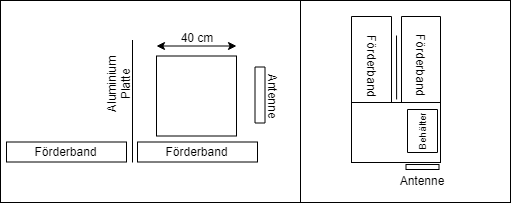
\includegraphics[keepaspectratio,width=\linewidth]{Positionierung_Antennen}
	\caption{Antennenposition Eins und Zwei}
	\label{fig:positionAntennen}
\end{figure}


Durch die Ausrichtung der Antennen wird weiter vorausgesetzt, dass das Lesegerät mit den Antennen eine maximale Distanz von 53.85cm lesen können. Jeder Behälter enthält gemäss Angaben im Normalfall 50 Exemplare. Daraus ergibt sich, dass das Lesegerät für den Normalfall mindestens 50 Exemplare in der Zeit auslesen muss, welche das Förderband benötigt um die Kiste ca. 60cm weit zu transportieren.

\section{Vergleich der vorgeschlagenen Lösung und der existierenden Situation}
Die existierende Situation enthält momentan noch keine Möglichkeit der Verifikation des Inhaltes eine Behältnisses. Demnach würde durch die Durchführung dieses Projektes die Wahrscheinlichkeit des Deplatzieren massiv verringern.

\section{Vorteile und deren Gründe der vorgeschlagenen Lösung}
\begin{itemize}
	\item Durch die Rückbeziehung, welche mittels der Mehrheit der gelesenen Tags auf die ID der Behälter zulässt, kann auf ein Barcodeleser verzichtet werden. Dies ermöglicht eine Positionsunabhängige Erkennung des Behälters.
	\item Die direkte Aussortierung des Behälters bringt mehrere Vorteile. So wird bereits der bestehende Prozess, mit welchem die Mitarbeiter vertraut sind, verwendet. Dies führt weiter zu dem Umstand, dass keine weiteren Fehlerquellen durch zusätzliche manuelle Interaktion durch einen Mitarbeiter, entstehen. Ein weiterer Vorteil liegt darin, dass die Erkennung sehr Früh geschieht, da die Aussortierung noch vor der Einlagerung des Behälters stattfindet.
	\item Der Einsatz mehrerer Antennen bringt den Vorteil, dass Tags mit verschiedenen Ausrichtungen identifiziert werden können. Dies aus dem Grund, dass sich die Tags bei unterschiedlichen Ausrichtungen unterschiedlich stark beeinflussen. Weiter kann durch den Einsatz mehrere Antennen der Suchradius vergrössert werden. Dies führt zu dem Umstand, dass sich der Behälter länger in einem Suchradius befindet, wodurch mehr Zeit für die Inventarisierung der Tags zur Verfügung steht. Deshalb können insgesamt mehr Tags identifiziert werden.
	\item Die Installation der RFID Antennen soll unmittelbar bei der Wiegestation erfolgen. Dies bringt den Vorteil, dass mehr Zeit für die Inventarisierung zur Verfügung steht, da der Behälter für eine kurze Zeit auf der Waage still steht. Weiter ist mit keiner Interferenz durch andere Behälter oder Objekte, wie Metall, zu rechnen, da sich nur Luft zwischen der Antenne und dem Behälter befindet.
\end{itemize}


\section{Vorgeschlagene Zulieferungsquellen}
Als Zulieferungsquellen für die RFID Hardware wird zu Feig Electronis geraten, da dieser Hersteller im Vergleich mit weiteren in Europa ansässigen Unternehmen ein gutes Preisleistungsverhältnis aufzeigt. Weiter spricht auch der Umstand, dass RFID Lösungsanbieter wie Bibliotheka auf Feig Electronis als Hersteller vertrauen, für Feig.

Für die Anpassung der Lagerverwaltungssoftware muss aufgrund der bestehenden Infrastruktur auf Stöcklin zurückgegriffen werden.

Die Umsetzung des Projektes soll, bedingt durch das vorhandene Lernpotential sowie tiefe Kosten, durch eine weitere Bachelorarbeit an einer Hochschule umgesetzt werden.

\section{Geschätzte Kosten und Quellen für die Basis dieser Schätzungen}
\subsection{Hardware}
\begin{tabularx}{\textwidth}{|r|X|r|r|}
	\hline
	\textbf{Menge} & \textbf{Produkt} & \textbf{Kosten(CHF)} & \textbf{Kosten gesamt(CHF)} \\
	\hline
	1 & RFID Reader ID ISC.LR2500-A (Feig) & 1'300 & 1'300 \\
	\hline
	2 & RFID Antennen ID ISC.ANT800/600 (Feig)& 830 & 1'660 \\
	\hline
	2 & RFID Antennenkabel ID ISC.ANT.C-A (Feig) & 22 & 44 \\
	\hline
	1 & RFID Multiplexer 8-fach HF Multiplexer (Feig) & 540 & 540 \\
	\hline
	1 & Netzteil ID NET.24V-B (Feig) & 33 & 33 \\
	\hline
	1 & Netzkabel ID CAB.NET.24V-B-EU (Feig) & 5 & 5 \\
	\hline
	1 & Raspberry Pi 3 Model B+ (pi-shop.ch)& 39 & 39 \\
	\hline
	1 & Sandisk Extreme 128GB Class 10 (digitec.ch)& 45 & 45 \\
	\hline
	& & & \textbf{3378} \\
	\hline
\end{tabularx}

Die Kosten dieser Schätzung aller Feig Electronics Artikel basieren auf der eingeholten Offerte (Siehe Abbildung \ref{fig:offerteFeig}), bei welcher EUR in CHF mit einem Wechselkurs von 1.14 auf welchem noch 8\% MwSt. Hinzugerechnet wurden.
Für die weiteren Artikel wurden auf den entsprechenden Seiten die Kosten verwendet (Besuch der Seite am 08.05.2019).

\begin{figure}[h!]
	\centering
	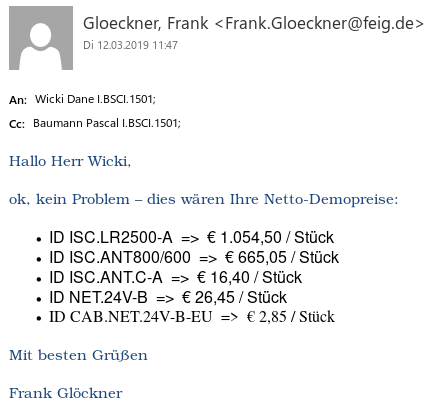
\includegraphics[keepaspectratio,width=.5\linewidth]{Screenshot_Email_Feig}
	\caption{E-Mail der Offerte}
	\label{fig:offerteFeig}
\end{figure}

\subsection{Software}
\begin{tabularx}{\textwidth}{|r|r|X|r|}
	\hline
	\textbf{Stunden(h)} & \textbf{Lohn(CHF/h)} & \textbf{Beschrieb} & \textbf{Kosten gesamt(CHF)} \\
	\hline
	50 & 200 & Umsetzung, sofern die Software die Befehle bereits über das Netzwerk entgegennimmt. & 10'000 \\
	\hline
	250 & - & Umsetzung des Projektes von einem Studenten im Rahmen einer Bachelorarbeit & 1'000 \\
	& & & \textbf{11'000} \\
	\hline
\end{tabularx}

Die Stundenkosten basieren auf aufgerundeten Werten, welche ein Freelancer in der Schweiz verdienen kann.
Für die Kosten der Bachelorarbeit wurden die Kosten übernommen, welche die Hochschule Luzern für deren Durchführung für eine Bachelorarbeit mit einem einzelnen Studenten
verrechnet.



\chapter{Entwicklungsplan}

\section{Kritische Punkte in der Entwicklung}
Es wurden vier kritische Punkte für die Entwicklung des Produktes identifiziert:
\begin{enumerate}
	\item Kickoff und Initialisierung
	\item Ausarbeitung Konzept
	\item Entwicklung und Implementierung
	\item Test und Abnahme
\end{enumerate}

\subsection{Initialisierung}
In dieser Phase soll die Planung erstellt werden, die Hardware beschafft und sich in das erarbeitete Konzept eingearbeitet werden. Weiter soll mit der Stöcklin durch die Teammitglieder oder den Kunden Kontakt aufgenommen und das Ausschleusen abgeklärt werden. Weiter soll in dieser Phase evaluiert werden, in welcher Programmiersprache die Lösung entwickelt wird.

\subsection{Ausarbeitung Konzept}
In dieser Phase sollen eventuelle Unklarheiten aus dem übergebenen Konzept, welche der erfolgreichen Durchführung im Weg stehen, abgeklärt und eliminiert werden. Es soll eine Architektur entwickelt werden und eine CI/CD Pipeline eingerichtet werden. Am Ende dieser Phase soll an Stöcklin der Auftrag erteilt werden, nötige Anpassung vorzunehmen und die Schnittstelle zu spezifizieren.

\subsection{Entwicklung und Implementierung}
In dieser Phase soll die Software entwickelt werden und unter Laborbedingungen an der Hochschule selber getestet werden. Vier Wochen nach Beginn dieser Phase soll von Stöcklin die Schnittstelle zur Ausschleusung eines Behälters zur Verfügung gestellt werden.

\subsection{Test und Abnahme}
In dieser letzten Phase soll die entwickelte Lösung beim Kunden installiert und getestet werden. Nachdem die Implementierung in das bestehende System der Stöcklin abgeschlossen ist, wird die Lösung durch den Kunden abgenommen.

\section{Kontrollprozesse für die Entwicklung}
Nach jeder abgeschlossenen Phase soll mit dem Kunden, der Speicherbibliothek, ein Meeting durchgeführt werden, bei dem die erarbeiteten Resultate präsentiert werden, das nächste Vorgehen besprochen und vom Kunden kontrollierend eingegriffen werden kann. Zur Kontrolle für beide beteiligten Parteien soll für jede Sitzung ein Protokoll angefertigt werden, welches bei der nächsten abgenommen wird.


\chapter{Kapitalvoraussetzungen und Investitionsplan}
Für die Umsetzung dieses Projektes muss in Folgendes investiert werden:

\vspace{1em}

\begin{tabularx}{\textwidth}{|X|r|}
	\hline
	\textbf{Beschreibung} & \textbf{Kosten (CHF)} \\
	\hline
	RFID Reader ID ISC.LR2500-A \footnote{\label{fn:HardwareKosten}Berechnung der Hardwarekosten (siehe Kapitel \ref{ssec:HardwareKosten})} & 1'300 \\
	\hline
	RFID Antennen ID ISC.ANT800/600 \footnotemark[1] & 1'660 \\
	\hline
	RFID Antennenkabel ID ISC.ANT.C-A \footnotemark[1] & 44 \\
	\hline
	RFID Multiplexer 8-fach HF Multiplexer \footnotemark[1] & 540 \\
	\hline
	Netzteil ID NET.24V-B \footnotemark[1] & 33 \\
	\hline
	Netzkabel ID CAB.NET.24V-B-EU \footnotemark[1] & 5 \\
	\hline
	Montagehalterung \footnotemark[1] & 250 \\
	\hline
	Softwareanpassungen Stöcklin \footnote{Berechnung der Softwarekosten (siehe Kapitel \ref{ssec:SoftwareKosten})} & 10'000 \\
	\hline
	Durchführung des Projektes Mitarbeiterkosten \footnote{Beschreibung der Mitarbeiterkosten (siehe Kapitel \ref{sec:MaterialMitarbeiterKosten})}  & 6'500 \\
	\hline
	\hline
	 & \textbf{20'332} \\
	 \hline
\end{tabularx}

\vspace{1em}

Um das Projekt durchführen zu können wird demnach ein Mindestkapital von 20'332 Franken vorausgesetzt.

\chapter{Geschätzte Betriebskosten und Ertrag}
Die Betriebskosten setzen sich aus zwei Faktoren zusammen
\begin{enumerate}
	\item Stromkosten der elektronischen Geräte
	\item Personalkosten bei einer fehlerhaften Erkennung
\end{enumerate}

Die Stromkosten werden durch einen Verbraucher erzeugt, dem RFID HF Lesegerät. Dieses Gerät konsumiert 35 Watt (\cite{DatenblattRFIDReader}). Dies entspricht bei einem stündigen Betrieb 35 W/h. Wird dieses Gerät während 365 Tagen ununterbrochen verwendet, resultiert daraus ein Stromverbrauch von 306.6 kW/h. Bei ungefähr 20 Rappen pro kW/h (\cite{StromPreisAdmin2019}) entspricht dies rund 61.30 Franken, welche jedes Jahr fällig werden ist.

Bei einer fehlerhaften Erkennung würden weitere Betriebskosten entstehen. Ein geschulter Mitarbeiter benötigt gut 20 Minuten, um den Behälter zu überprüfen und festzustellen, dass es sich bei der Aussortierung um einen Fehler handelt.

Unter der Annahme, dass dieser Fall jeden Monat bis zu viermal geschehen würde, bräuchte der Mitarbeiter rund 16h pro Jahr für die Identifizierung einer fehlerhaften Erkennung. Dies entspricht rund 1'135.7 Franken bei einer Vollkostenrechnung eines Mitarbeiters mit einem Lohn von ca. 6'000 Franken (\cite{KostenProMitarbeiter2013}).

Zusammen ergibt dies Jährliche kosten von rund 1'196 Franken.

Die möglichen Einsparungen entstehen durch das Fernbleiben einer aufwendigen Suche nach einem Einzelexemplar. Diese würde sich wie folgt zusammensetzen:
Bei 110'000 Behälter bräuchte man durchschnittlich gesehen rund 55'000 Versuche, um das Exemplar zu finden. Die durchschnittliche Anzahl Durchsuchungen kann jedoch anhand von weiteren Informationen, welche dem Lagerverwaltungssystem bekannt sind, auf ca. 35'000 Versuche reduziert werden. Würde nun ein Mitarbeiter wieder 20 Minuten für die Durchsuchung eines Behälters benötigen, würde die Suche annähernd 12'000 Stunden andauern. Bei einem Mitarbeiter mit einem Lohn von 6'000 Franken würden die Gesamtkosten auf rund 852'000 Franken betragen.

Bei Kosten von 852'000 Franken für eine Suche nach einem einzelnen Exemplar würde dieses bei Bemerkung des Verlustes ersetzt werden, da eine Neubeschaffung in fast allen Fällen kostengünstiger und ökologischer ist. Sollte es sich jedoch um ein Unikat handeln, müsste dennoch dieser Suchprozess durchgeführt werden.

Weiter würde bei einer Deplatzierung eines Objektes die Reputation der Speicherbibliothek sowie das Vertrauen in diese nachhaltig Schaden nehmen.

Weiter ist zu bedenken, dass selbst bei einer Wahrscheinlichkeit von nur 0.000001\% einer Deplatzierung pro Einlagerung, bereits ein Exemplar pro Million Exemplare deplatziert werden würde.

\chapter{Wirtschaftliche Machbarkeit des Projekts}
Die Initialkosten von 20'332 Franken mit den weiteren Betriebskosten von 1'244.32 Franken pro Jahr dienen der Reduzierung eines menschlichen Fehlers im Einlagerungsprozess. Dank dieser Umsetzung kann das Risiko reduziert werden, dass ein Reputationsschaden entsteht, welcher schlimmstenfalls auch zu politischen Folgen führen kann.
Durch das Verhindern eben dieser negativen Folgen stellt sich der Nutzen klar über die Initialkosten von rund 20'332 Franken.

Für die initiale Phase der Realisierung, müssten finanzielle Ressourcen von rund 20'332 Franken benötigt. Für die Beschaffung dieser Finanzen ist alleine die Speicherbibliothek zuständig.

\section{Grösste Kosten und Risiken}
Die grössten Kosten sowie auch Risiken entstehen bei der Anpassung des bestehenden Lagerverwaltungssystems, da zu dieser durch Stöcklin noch keine Informationen, bezüglich des Aufwandes, bekannt sind. Auch die Einhaltung der Zeitfrist von einem Monat für die Auslieferung der Schnittstellen ist aufgrund des fehlenden Wissens über die Software sowie die Kapazitäten des Unternehmens Stöcklin mit grösseren Risiken verbunden.

Ein weiteres Terminrisiko geht zudem vom Hardwarehersteller aus, da dieser unter Umständen eine längere Zeit für die Lieferung der Hardware benötigt.

Beide Terminrisiken können jedoch während der Implementation der Software weitestgehend abgefangen werden.


\newpage

\pagenumbering{Roman}

\appendix

\listoffigures

\printbibliography

\clearpage

\pagenumbering{gobble}

\chapter{Konzept}
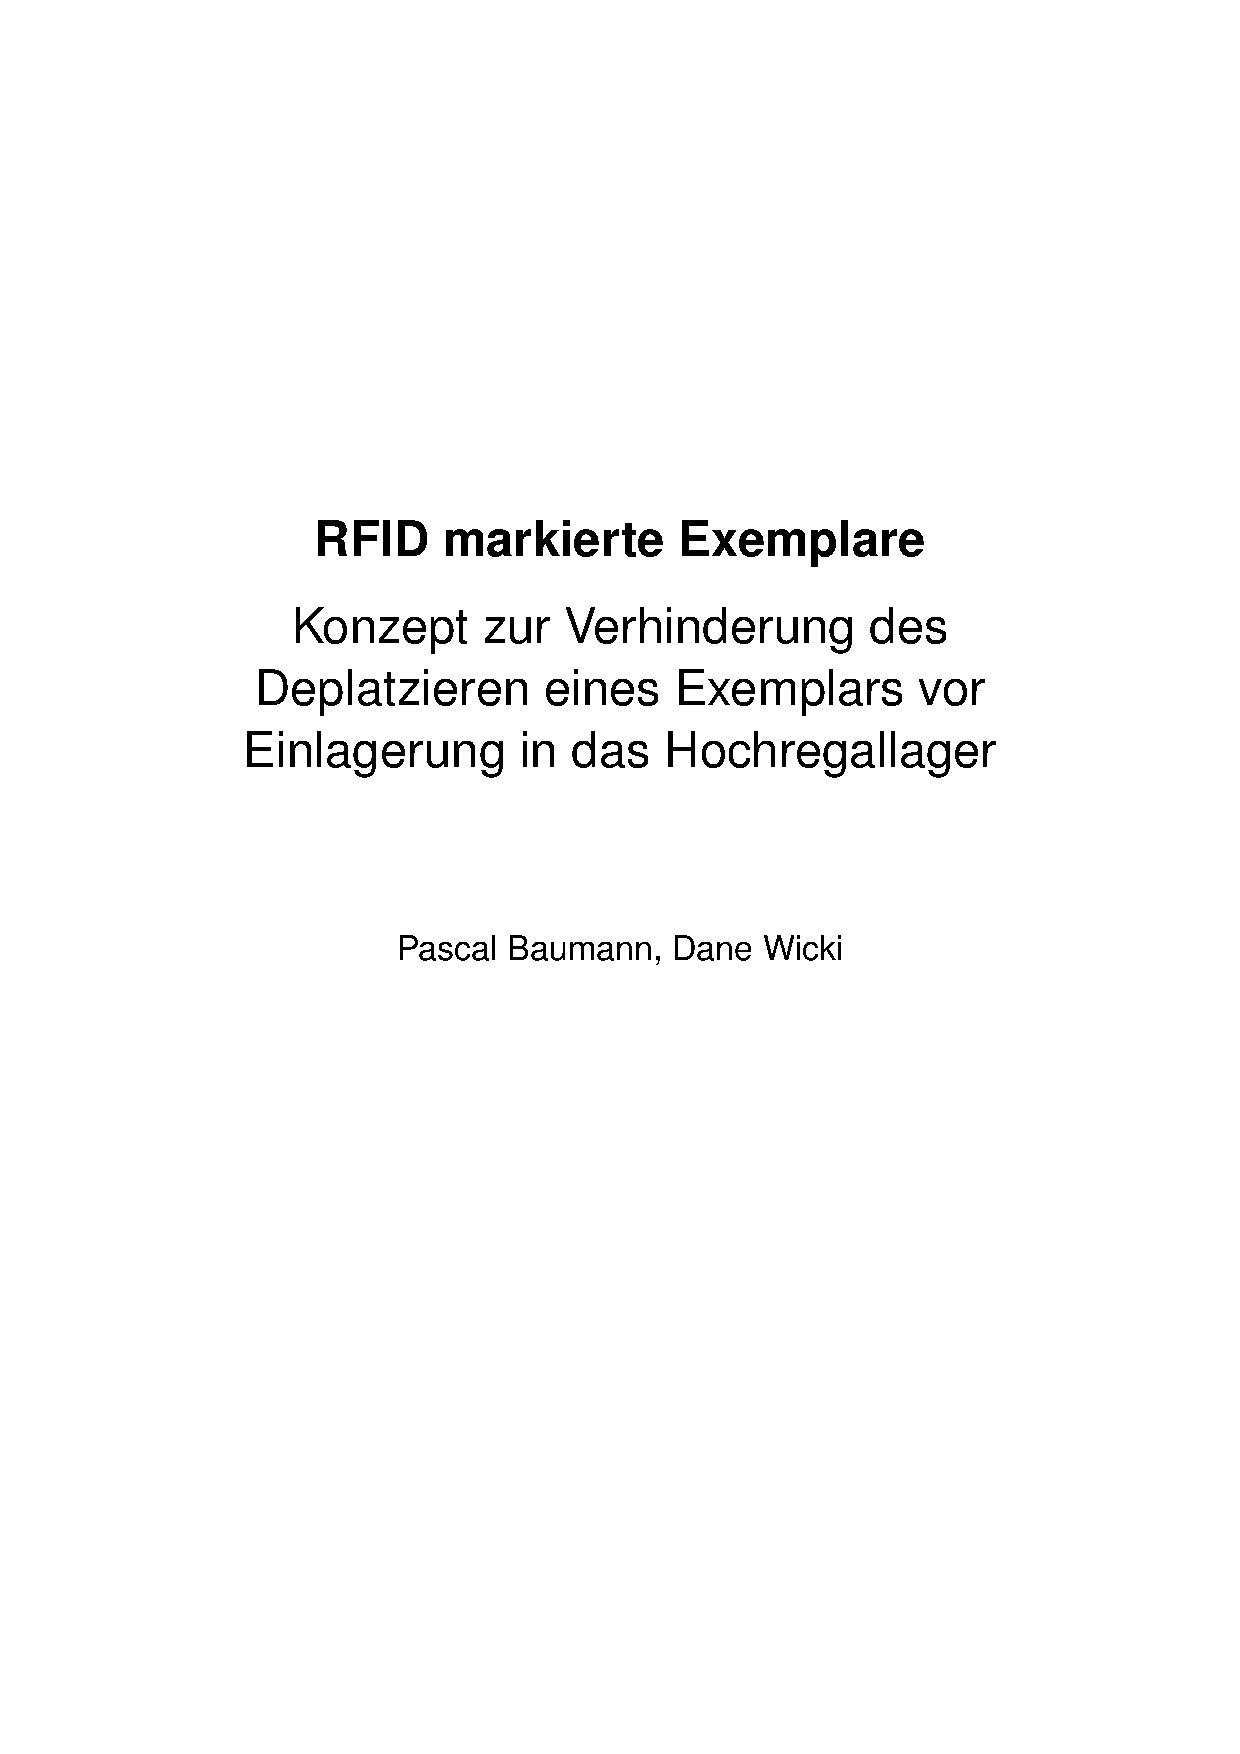
\includepdf[pages=-]{appendix/Zweites_Konzept_Hauptdatei.pdf}


\chapter{Versuche}
\label{app:ch:Versuche}
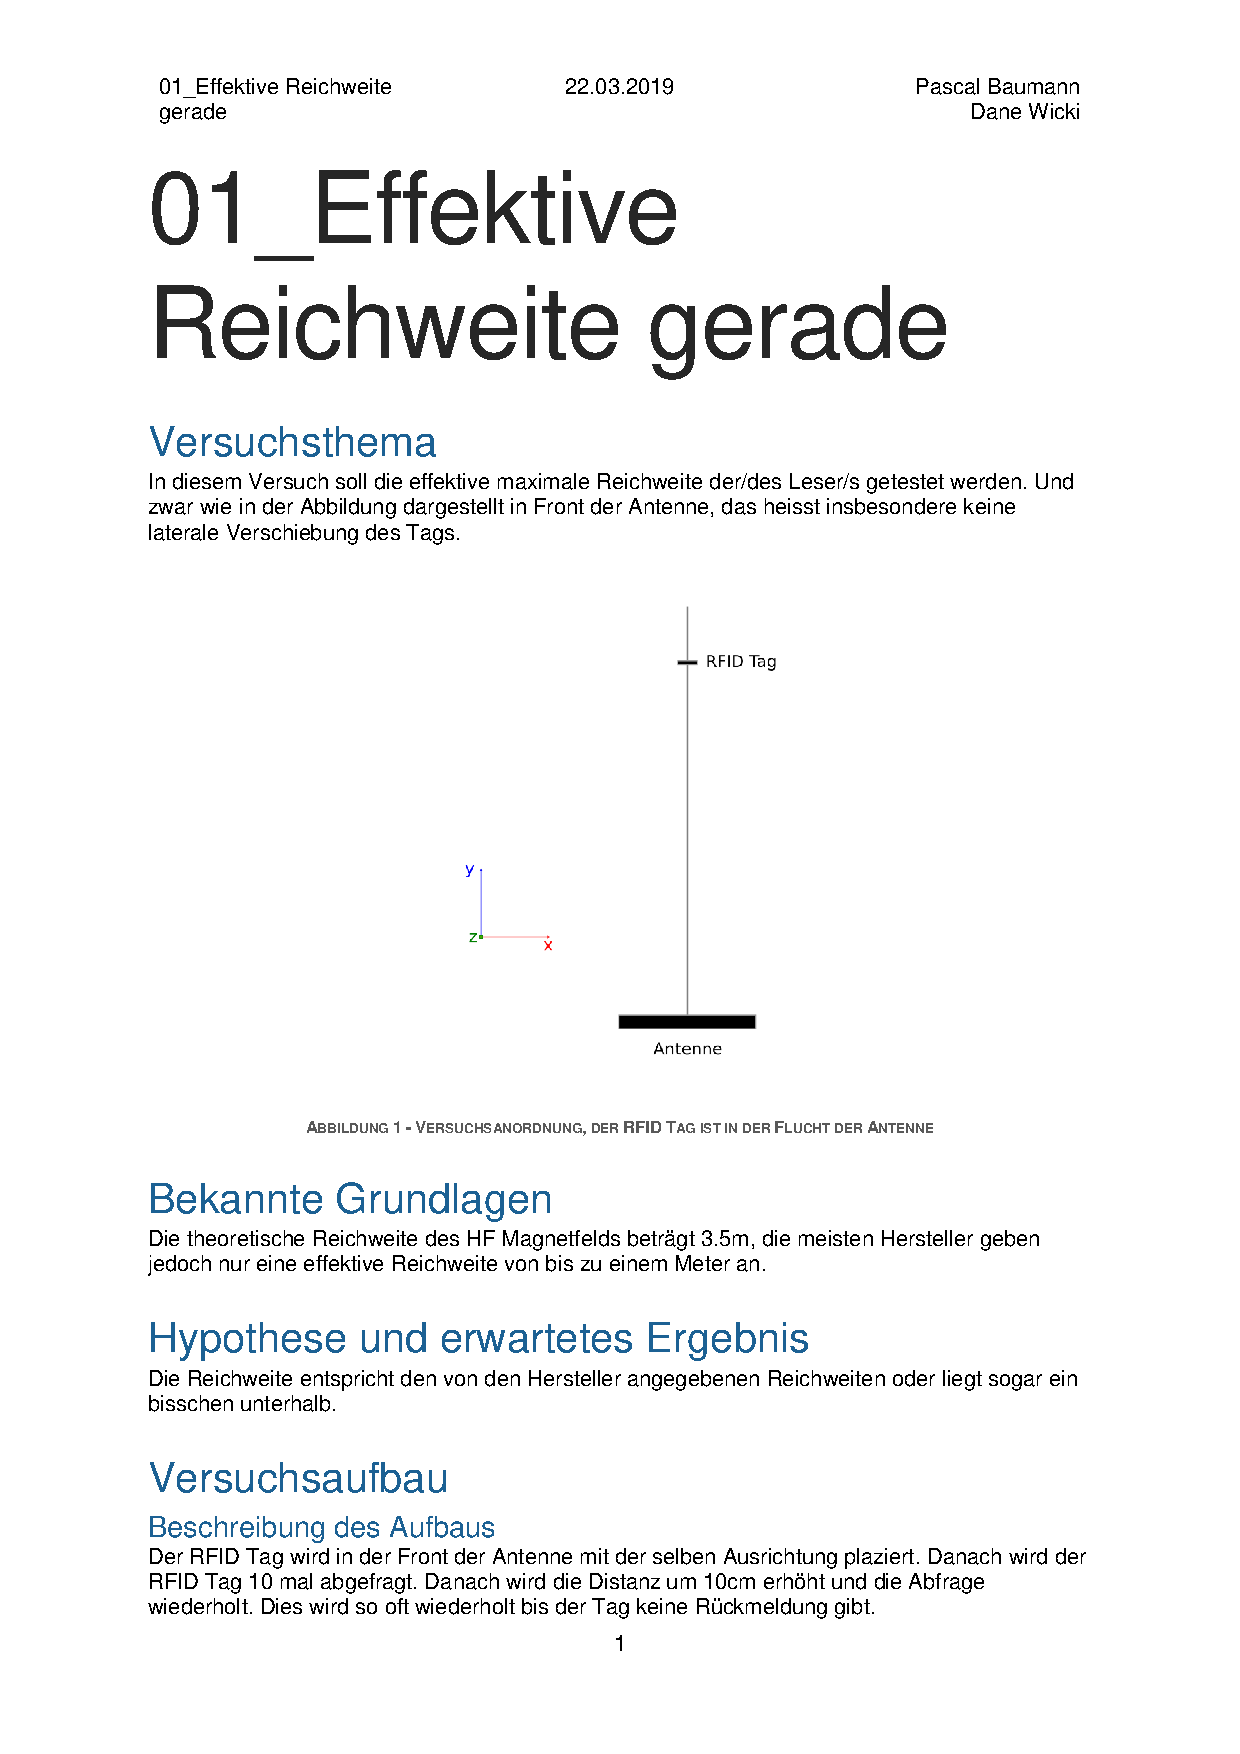
\includepdf[pages=-]{appendix/20190521Versuche.pdf}

\end{document}
